\chapter{Experiments\label{cha:chapter4}}
This chapter provides details about the experiments conducted within the context of this thesis. 


\section{Experimental Setup\label{sec:setup}}
All experiments are caried out on machine XYZ. 

\section{Hyperparamter Tuning\label{sec:datasets}}

\section{Dataset-Specific Results\label{sec:datasets}}



%\section{Results for Experiment A\label{sec:results1}}
%Figure~\ref{fig:aliceandbob} illustrates the situation between Alice and Bob. (sequence diagram from www.websequencediagrams.com)

%\begin{figure}[htb]
%  \centering
%  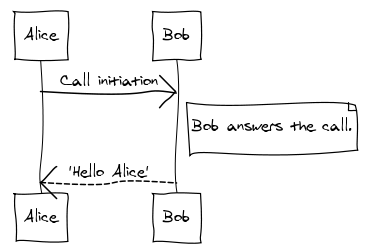
\includegraphics[width=9cm]{uml_seq_example.png}\\
%  \caption[Example figure]{Alice and Bob}
%  \label{fig:aliceandbob}
%\end{figure}

%\section{Results for Experiment B\label{sec:results2}}
%In Table~\ref{table:example} the statistics for...

%\begin{table}[H]
%  \begin{center}
%  \begin{tabular}{ | p {2.5cm}| p{3.6cm}| p{3.6cm}| p{3.3cm}| }
%  \hline
%  \textbf{Dateset} & \textbf{Minimum y} & \textbf{Maximum y} & \textbf{Average y} \\
%  \hline
%  DS 1 & -68.57 & 506.78 & 86.05 \\ \hline
%  DS 2 & -0.18 & 537.67 & 102.51 \\
%  \hline
%  \end{tabular}
%  \caption[Example table]{This table shows the statistics (minimum, maximum, and average) for the different datasets.}
%  \label{table:example}
%  \end{center}
%\end{table}


%\section{Discussion of Results\label{sec:resultDiscussion}}
%...
